\section{Predictive approach}
\label{exp:predictive}

This section presents performance results related to the evaluation of \pSPS{} and its ability to adapt to the dynamics of the data stream, without reducing the rate of processed events.

The evaluation is composed of six parts: (1) the impact of interval time (Section \ref{exp:pa-time}); (2) an analysis of predictive models (Section \ref{exp:pa-models}); (3) a comparison of \pSPS{} with the original Storm, using a fixed number of replicas (Section \ref{exp:pa-storm}) as well as with (4) the other predictive adaptive SPS, \textit{DABS-Storm}, proposed in \cite{KombiLLRB19} (Section \ref{exp:pa-dabs}); (5) an experiment with a complex application (Section \ref{exp:pa-complex}) and finally (6) with other datasets (Section \ref{exp:pa-dataset}).

\subsection{Impact of the time interval}
\label{exp:pa-time}
Aiming at tuning their value, we propose in this section to discuss the impact of the time interval ($td$) used in Equation \ref{eq:prediction-replicas} \footnote{In this experiment to calculate Equation \ref{eq:prediction-queue}, the dependence among operators was not considered, because it was tested with a previous version of the prediction model.}. We used the \textit{Twitter Smoothed} dataset, the \textit{Twitter linear - Classification} application, the \textit{Basic} model for input prediction, and \textit{Load-Aware grouping} for stream grouping strategy. For calculating the \textit{Saved resources} metric, we have fixed $r_{over} = 32$ (i.e., $r_i = 8$).

%% Note Daniel: There is a difference between this evaluation and the following ones, as this one was conducted in SBAC and the following ones for JPDC.

Table \ref{tab:exp-pa-time} shows the values of the four metrics when the value of $td$ varies.
Note that the greater the time interval, the greater the number of samples used for calculating Equation \ref{eq:prediction-replicas}. We observe an improvement in the results when the time interval is small, which is also in accordance with the dynamic behavior of the input rate. Latency and throughput degradation confirm the latter, given that by increasing $td$ the system needs to wait longer to adjust the number of replicas and stabilize. 

It is important to highlight that, unlike Storm's traditional solution, which must restart the application to reconfigure the number of resources of each operator, \pSPS{} should only activate or deactivate replicas in the pool. Therefore, the reconfiguration downtime does not exist. Furthermore, the computational cost of calculating the equations is minimal since they are basic operations carried out by the system. Consequently, even if reconfiguration occurs quite often, we do not observe a decrease in the number of processed events.

\begin{table}[!ht]
\centering
\begin{tabular}{|l|llll|}
\hline Time interval
& \begin{tabular}[c]{@{}l@{}}Saved\\ Resources\end{tabular} & \begin{tabular}[c]{@{}l@{}}Throughput\\ Degradation\end{tabular} & \begin{tabular}[c]{@{}l@{}}Diff. Proc.\\ Events\end{tabular} & \begin{tabular}[c]{@{}l@{}}Latency\\ (ms)\end{tabular} \\ \hline \hline
$td=30s$      & 0.5617   & 0.1831 & 0.9987 & 2098.91 \\ \hline
$td=60s$      & 0.5390   & 0.4332 & 0.9979 & 5271.01 \\ \hline
$td=120s$      & 0.5219   & 0.9221 & 0.9976 & 17068.33 \\ \hline
$td=180s$      & 0.5563   & 0.8028 & 0.9992 & 22364.86 \\ \hline
\end{tabular}
\caption{System metric values with different time intervals using \textit{Twitter Smoothed}.}
\label{tab:exp-pa-time}
\end{table}

\subsection{Comparison of predictive models}
\label{exp:pa-models}
We propose in this section to discuss the use of predictive models for the calculation of the number of events sent by input data ($\widehat{\lambda_G}(t+1)$) and their impact on system performance. We used the \textit{Twitter Smoothed} dataset, the \textit{Twitter linear - Classification} application, and \textit{Load-Aware grouping} for stream grouping strategy. For calculating the \textit{Saved resources} metric, we have fixed $r_{over} = 32$ (i.e., $r_i = 8$).

\begin{table}[!ht]
\centering
\begin{tabular}{|l|llllll|}
\hline \begin{tabular}[c]{@{}l@{}}Pred.\\ Model\end{tabular} & \begin{tabular}[c]{@{}l@{}}Saved\\ Resources\end{tabular} & \begin{tabular}[c]{@{}l@{}}Throughput\\ Degradation\end{tabular} & \begin{tabular}[c]{@{}l@{}}Diff. Proc.\\ Events\end{tabular} & \begin{tabular}[c]{@{}l@{}}Latency\\ (ms)\end{tabular} & \begin{tabular}[c]{@{}l@{}}Error Est.\\ Input\end{tabular} & \begin{tabular}[c]{@{}l@{}}Error Est.\\ Replica\end{tabular} \\ \hline \hline
ANN   & 0.475 & 0.070 & 1.000      & 355.490  & 0.212 & 0.277 \\ \hline
FFT   & 0.519 & 0.189 & 1.000      & 1023.380 & 0.249 & 0.345 \\ \hline
LR    & 0.533 & 0.195 & 1.000      & 663.030  & 0.090 & 0.140 \\ \hline
RF    & 0.538 & 0.227 & 0.996      & 583.921  & 0.140 & 0.193 \\ \hline
Basic & 0.560 & 0.325 & 1.000      & 1295.490 & 0.180 & 0.287 \\ \hline
\end{tabular}
\caption{System metric values of different predictive models using \textit{Twitter Smoothed}.}
\label{tab:exp-pa-models}
\end{table}

For each predictive model, Table \ref{tab:exp-pa-models} shows the respective values for the above discussed metrics.
There is no difference in processed events, except for the \textit{RF} model that presents a slight decrease in the number of processed events, representing a loss of only $0.4\%$ of the incoming events. Therefore, we all models are reliable to be used in whole event processing experiments.

We can also observe that \textit{ANN} has the lowest latency, with a difference of $39.12\%$ compared to the second lowest latency model (\textit{RF}). Such values mean that \pSPS{} using \textit{ANN} processes the received events faster than the others. However, in this case, it needs a larger amount of resources, as shown by the saved resources metric, where \textit{ANN} has the lowest value, i.e., $15.17\%$ worse than the \textit{Basic} model metric. Thus, there is a trade-off between latency and the amount of resources: on the one hand, if the requirement is a SPS that processes all incoming events with low latency, \textit{ANN} is the most suitable model; on the other hand, if the aim is the reduction of costs and the loss of events is not an issue, having an acceptable latency, \textit{RF} is more suitable.

\begin{figure}[!ht]
    \centering
    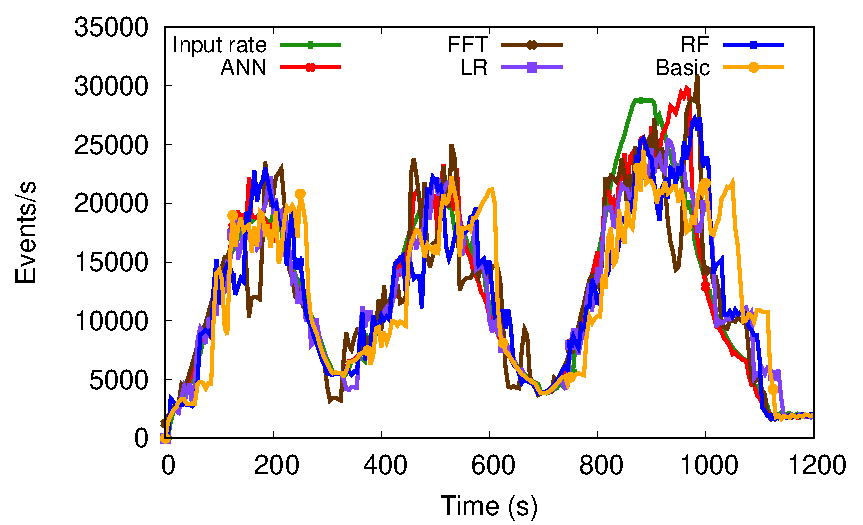
\includegraphics[width=0.75\linewidth]{figures/exp/predictive/TwitterLinear-Models-Throughput.pdf}
    \caption{Throughput of \pSPS{} using different predictor models.}
    \label{fig:exp-pa-models-throughput}
\end{figure}

Regarding the estimation error of the input rate and number of replicas, a lower estimation error can not be interpreted as better performance.
Overestimating the input rate implies an overestimation of the number of replicas, using a larger amount of resources. Consequently, more replicas are available for event processing as shown in Figure \ref{fig:exp-pa-models-throughput}.

Conversely, if the number of replicas is underestimated, the margin for processing events is smaller, making it more likely that events will be stuck and the system will be more unstable. 
In this case, events will probably get stuck in queues, making the SPS more unstable.
Regarding accuracy, \textit{LR} has the best one with an improvement of $57.54\%$ over \textit{ANN}, which does not mean that it present better performance, because there are moments when underestimating the number of replicas decreases the processing of events in the execution of the system. Unlike \textit{ANN} that presents an overprovisioning of resources whenever the curve rises. On the other hand, in \textit{FFT}, its estimation error has a strong impact in \pSPS{} performance since it does not accurately predict the behaviour of the input rate, as shown in Figure \ref{fig:exp-pa-models-replicas}.

\begin{figure}[!ht]
    \centering
    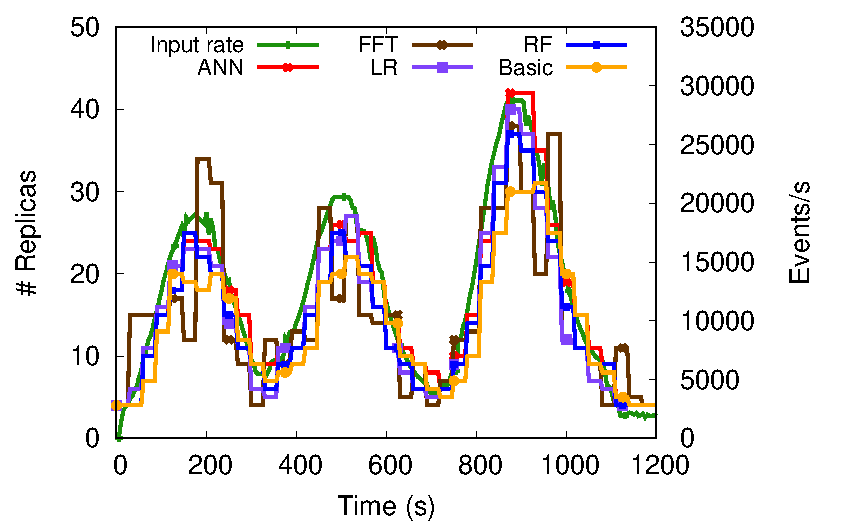
\includegraphics[width=0.75\linewidth]{figures/exp/predictive/TwitterLinear-Models-Replicas.pdf}
    \caption{Total number of replicas of \pSPS{} using different predictor models.}
    \label{fig:exp-pa-models-replicas}
\end{figure}


\subsection{Comparison of \pSPS{} with Storm}
\label{exp:pa-storm}
This section compares \pSPS{} with the original \textit{Storm} where the number $r$ of replicas per operator is fixed. We have considered three configurations for \textit{Storm}: no replication ($r=1$); four replicas ($r=4$); eight replicas ($r=8$). The latter corresponds to the \textit{overprovisioning} configuration where the total number of replicas, $r_{over} = 32$ (i.e., $r_i = 8$), same value used to calculate \textit{Saved resources}. The total number of replicas of each configuration is shown in Figure \ref{fig:exp-pa-storm-replicas}. We used the \textit{Twitter Smoothed} dataset, the \textit{Twitter linear - Classification} application, the \textit{ANN} model for input prediction, and \textit{Load-Aware grouping} for stream grouping strategy.

\begin{figure}[!ht]
     \centering
     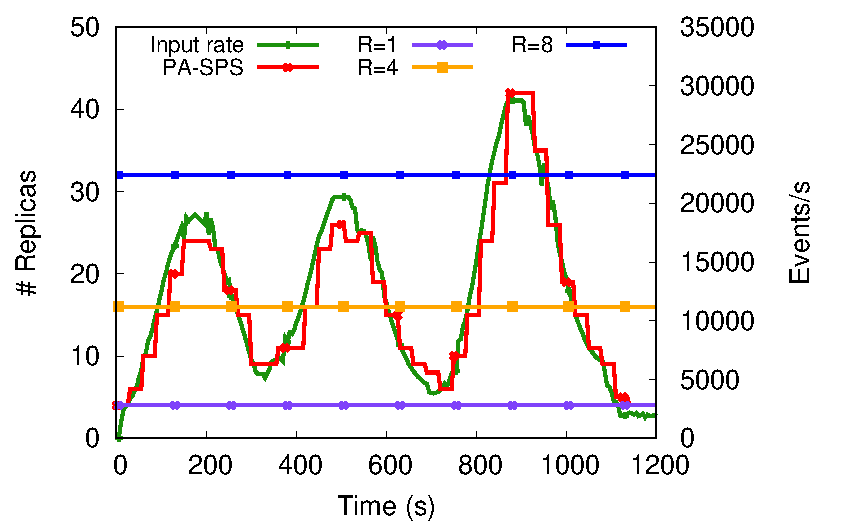
\includegraphics[width=0.75\linewidth]{figures/exp/predictive/TwitterLinear-Storm-Replicas.pdf}
     \caption{Total number of replicas using \textit{\pSPS{}} and different configurations in \textit {Storm}.}
     \label{fig:exp-pa-storm-replicas}
\end{figure}

Table \ref{tab:exp-pa-storm} summarizes the results of the different configurations. We observe that the system without replication ($r=1$) has a very low performance, because it only processes $33.1\%$ of the incoming events (see Figure \ref{fig:exp-pa-storm-throughput}). Such a result is due to the lack of adaptation when incoming events increase. Consequently, there exists a bound for the number of events to process while the others are queued. 
Therefore, although such a configuration presents low resource usage, it is not recommended for performance sake.

\begin{table}[!ht]
\centering
\begin{tabular}{|l|llll|}
\hline System
& \begin{tabular}[c]{@{}l@{}}Saved\\ Resources\end{tabular} & \begin{tabular}[c]{@{}l@{}}Throughput\\ Degradation\end{tabular} & \begin{tabular}[c]{@{}l@{}}Diff. Proc.\\ Events\end{tabular} & \begin{tabular}[c]{@{}l@{}}Latency\\ (ms)\end{tabular} \\ \hline \hline
\pSPS{}     & 0.475   & 0.071 & 1.000      & 355.490   \\ \hline
$r=1$           & 0.875   & 0.515 & 0.331 & 196962.950 \\ \hline
$r=4$           & 0.500      & 0.855 & 0.987 & 269.750    \\ \hline
$r=8$           & 0.000     & 0.000   & 1.000   & 153.510    \\ \hline
\end{tabular}
\caption{System metric values with \textit{\pSPS{}} and different configurations in \textit {Storm} using \textit{Twitter Smoothed}.}
\label{tab:exp-pa-storm}
\end{table}

On the other hand, the $r=4$ configuration has only a $1.3\%$ difference between incoming and processed events. 
The decrease in the amount of resources by $50\%$ increases latency by $43.03\%$. Thus, once again, there is a tradeoff between performance and used resources, corroborating to our previous discussion.

Finally, \pSPS{}  decreases by $5\%$ Saved Resources with respect to $r=4$, but it is able to process all incoming events. Compared to the $r=8$ configuration \pSPS{} presents: (1) a $131.57\%$ higher latency, whose impact should be balanced with its ability to dynamically adapt itself; (2) a difference of $7.01\%$ in throughput degradation, which means that it greatly adapts itself in order to process most of incoming events (see Figure \ref{fig:exp-pa-storm-throughput}).

\begin{figure}[!ht]
     \centering
     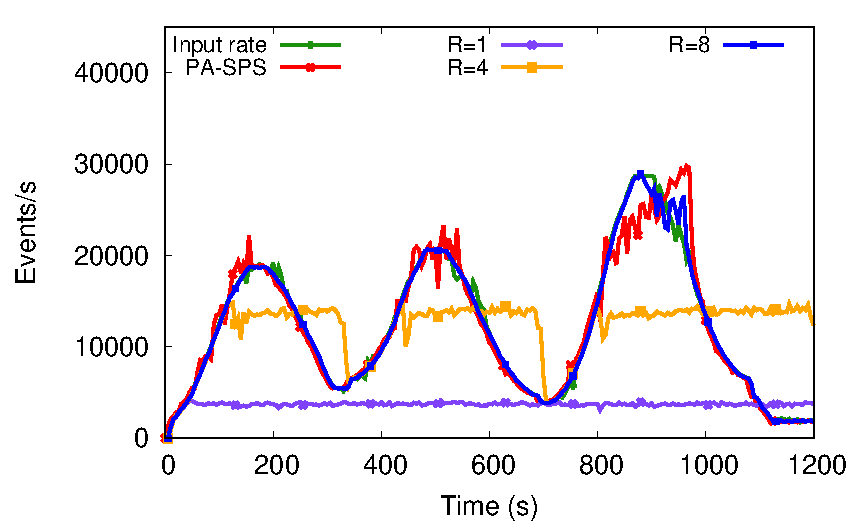
\includegraphics[width=0.75\linewidth]{figures/exp/predictive/TwitterLinear-Storm-Throughput.pdf}
     \caption{Throughput using \textit{\pSPS{}} and different configurations in \textit {Storm}.}
     \label{fig:exp-pa-storm-throughput}
\end{figure}

\subsection{Comparison between \pSPS{} and DABS-Storm}
\label{exp:pa-dabs}
The aim of this experiment is to compare \pSPS{} with \textit{DABS-Storm} (denoted \textit{DABS}), proposed in \cite{KombiLLRB19} (see Section \ref{rw-auto-predictive}). We used the \textit{Twitter Smoothed} dataset, the \textit{Twitter linear - Classification} application, the \textit{ANN} model for input prediction, and \textit{Load-Aware grouping} for stream grouping strategy. For calculating the \textit{Saved resources} metric, we have fixed $r_{over} = 32$ (i.e., $r_i = 8$).

\begin{table}[!ht]
\centering
\begin{tabular}{|l|llll|}
\hline System
& \begin{tabular}[c]{@{}l@{}}Saved\\ Resources\end{tabular} & \begin{tabular}[c]{@{}l@{}}Throughput\\ Degradation\end{tabular} & \begin{tabular}[c]{@{}l@{}}Diff. Proc.\\ Events\end{tabular} & \begin{tabular}[c]{@{}l@{}}Latency\\ (ms)\end{tabular} \\ \hline \hline
\pSPS{}     & 0.475   & 0.071 & 1.000 & 355.490   \\ \hline
%PSPS              & 0.561   & 0.183 & 0.998 & 2098.910 \\ \hline
DABS              & 0.396   & 0.284 & 0.828 & 1391.280 \\ \hline
\end{tabular}
\caption{System metric values of \pSPS{} and DABS using \textit{Twitter Smoothed}.}
\label{tab:exp-pa-dabs}
\end{table}

Table \ref{tab:exp-pa-dabs} gathers the metric values related to \pSPS{} and DABS. PA-SPS is able to process all events, but not \textit{DABS} as shown in Figure \ref{fig:exp-pa-dabs-throughput}. The latter decreases by $17.2\%$ the number of events processed. Similarly to \textit{Storm} (see Section \ref{pool}), \textit{DABS} needs to restart the application for reconfiguring the number of replicas, which is not the case of \pSPS{} due to their pool of replicas. Therefore, downtime has an impact in the number of events that are processed.

As we have already discussed, the increase of resources has a correlation with the decrease of latency, but there are scenarios where it does not apply. For example, in \textit{DABS}, saved resources have been decreased by $16.63\%$ when compared to \pSPS{}, but its latency is $291.36\%$ higher. Such a behavior can be explained since \textit{DABS} overestimates resources in non-critical intervals, as observed between $t=800s$ and $t=900s$ in Figure \ref{fig:exp-pa-dabs-replicas}, which is useless in the case of curve peaks, where more resources are needed.

\begin{figure}[!ht]
    \centering
    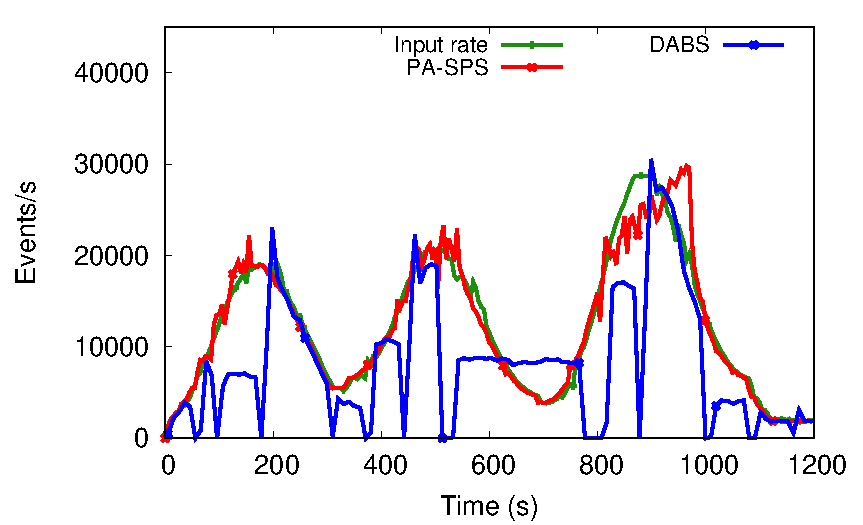
\includegraphics[width=0.75\linewidth]{figures/exp/predictive/TwitterLinear-RW-Throughput.pdf}
    \caption{Throughput using \textit{\pSPS{}} and \textit{DABS}.}
    \label{fig:exp-pa-dabs-throughput}
\end{figure}


\begin{figure}[!ht]
    \centering
    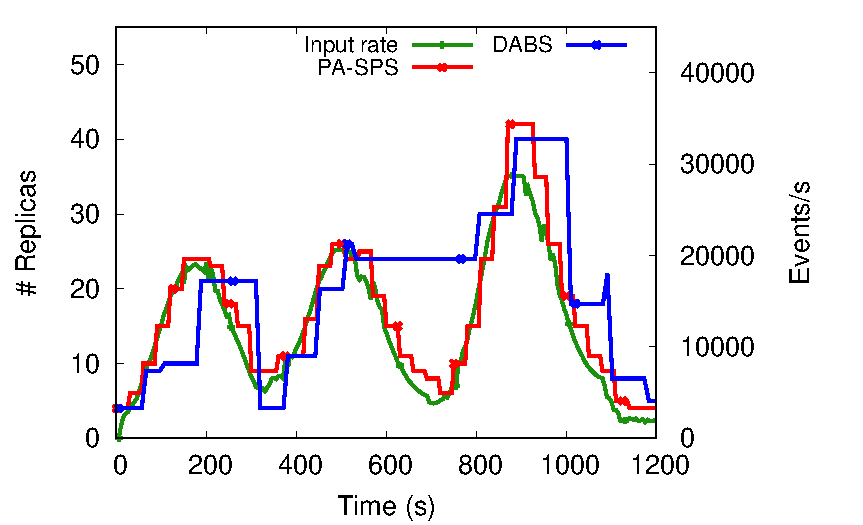
\includegraphics[width=0.75\linewidth]{figures/exp/predictive/TwitterLinear-RW-Replicas.pdf}
    \caption{Total number of replicas using \textit{\pSPS{}} and \textit{DABS}.}
    \label{fig:exp-pa-dabs-replicas}
\end{figure}

\subsection{Complex application}
\label{exp:pa-complex}
We have also evaluated \pSPS{} with a complex application. For this experiment, we have compared \pSPS{} with an overprovisioning Storm which always uses a fixed number of replicas per operator, denoted $S_{over}$. Such numbers are fixed ($r_i=5$) at the beginning of the data processing and do not vary during the experiment. We used the \textit{Twitter Smoothed} dataset, \textit{Twitter complex} application, and \textit{Load-Aware grouping} for stream grouping. For calculating the \textit{Saved resources} metric, we have fixed $r_{over} = 40$ (i.e., $r_i = 5$).

Table \ref{tab:exp-pa-complex-app} shows evaluation results obtained with \pSPS{} and Storm. In \pSPS{}, we observe a high reduction of used resources with $68.8\%$ fewer active replicas, when compared to Storm. Such a decrease has an impact on the physical used resources: CPU consumption of \pSPS{} (resp. Storm) is in average, $9.57\%$ (resp. $14.66\%$).
This difference happens because each replica is associated with a thread. Therefore, with a fixed number of 5 replicas, Storm requires more CPU than \pSPS{} where the number of replicas dynamically varies.

\begin{table}[!ht]
\hspace*{-0.5cm}
\centering
\begin{tabular}{|l|llll|}
\hline System & \begin{tabular}[c]{@{}l@{}}Saved\\ Resources\end{tabular} & \begin{tabular}[c]{@{}l@{}}Throughput\\ Degradation\end{tabular} & \begin{tabular}[c]{@{}l@{}}Diff. Proc.\\ Events\end{tabular} & \begin{tabular}[c]{@{}l@{}}Latency\\ (ms)\end{tabular}\\ \hline \hline
\pSPS{}   & 0.688  & 0.031 & 1.000  & 209.270 \\ \hline
$S_{over}$           & 0.000    & 0.000    & 1.000 & 31.990 \\ \hline
\end{tabular}
\caption{System metric values of \pSPS{} and $S_{over}$ using \textit{Twitter Smoothed} and Twitter complex application.}
\label{tab:exp-pa-complex-app}
\end{table}

\subsection{Other datasets}
\label{exp:pa-dataset}
The aim of this section is to evaluate our system with other datasets, to analyse its adaptability and the behaviour of the results according to the predictive model used.

\subsubsection{Twitter Raw}
We used the \textit{Twitter Raw} dataset, the \textit{Twitter linear - Classification} application, and \textit{Load-Aware grouping} for stream grouping strategy. For calculating the \textit{Saved resources} metric, we have fixed $r_{over} = 32$ (i.e., $r_i = 8$).

\begin{table}[!ht]
\centering
\begin{tabular}{|l|llllll|}
\hline \begin{tabular}[c]{@{}l@{}}Pred.\\ Model\end{tabular} & \begin{tabular}[c]{@{}l@{}}Saved\\ Resources\end{tabular} & \begin{tabular}[c]{@{}l@{}}Throughput\\ Degradation\end{tabular} & \begin{tabular}[c]{@{}l@{}}Diff. Proc.\\ Events\end{tabular} & \begin{tabular}[c]{@{}l@{}}Latency\\ (ms)\end{tabular} & \begin{tabular}[c]{@{}l@{}}Error Est.\\ Input\end{tabular} & \begin{tabular}[c]{@{}l@{}}Error Est.\\ Replica\end{tabular}\\ \hline \hline
ANN   & 0.395 & 0.213 & 1.000      & 1044.510  & 0.424 & 0.466 \\ \hline
FFT   & 0.153 & 0.579 & 1.000      & 12285.990 & 0.903 & 1.282 \\ \hline
LR    & 0.421 & 0.261 & 0.988   & 1366.680  & 0.397 & 0.391 \\ \hline
RF    & 0.539 & 0.381 & 0.987   & 2610.330  & 0.253 & 0.398 \\ \hline
Basic & 0.513 & 0.251 & 1.000      & 1049.490  & 0.312 & 0.407  \\ \hline
\end{tabular}
\caption{System metric values of different predictive models using \textit{Twitter Raw}.}
\label{tab:exp-pa-twitter-raw}
\end{table}

Table \ref{tab:exp-pa-twitter-raw} shows the results obtained, which have similar values with Table \ref{tab:exp-pa-models}, related to smoothed data. \pSPS{}, regardless the model, has processed most of the received events, with only $1.2\%$ (resp., $1.3\%$) of events not processed by \textit{LR} (resp., \textit{RF}). Also, the lowest latency corresponds to \textit{ANN}, although the difference in latency with respect to the second best model (\textit{Basic}) is $0.47\%$.

\begin{figure}[!ht]
     \centering
     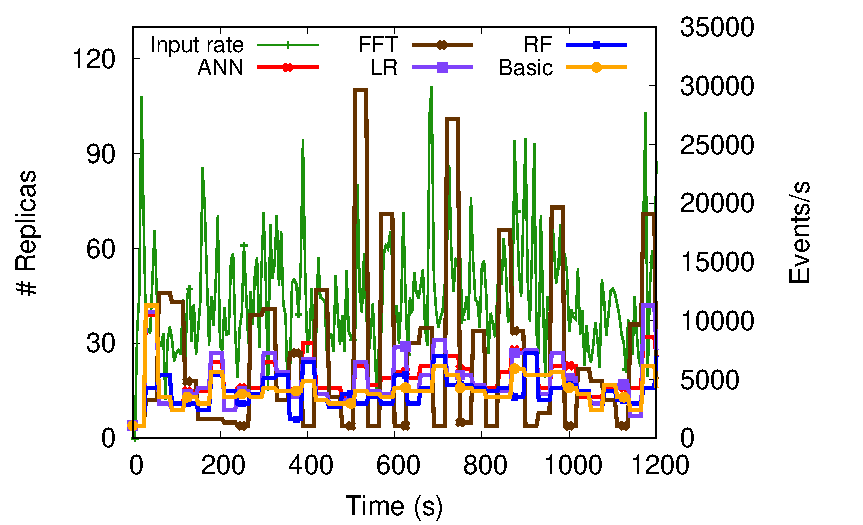
\includegraphics[width=0.75\linewidth]{figures/exp/predictive/TwitterRaw-Replicas.pdf}
     \caption{Total number of replicas of \pSPS{} using \textit{Twitter raw} dataset.}
     \label{fig:exp-pa-twitter-raw-replicas}
\end{figure}


By using a more unstable input rate (see Figure \ref{fig:exp-pa-twitter-raw-throughput}), the estimation error of the models increases as the input behaviour is more complex to predict. Since \pSPS{} also becomes more unstable, the throughput degradation increases. \textit{FFT} presents the  highest difference because the input rate does not have a stationary behaviour. Consequently, there is a large percentage of error in the prediction of the input and the number of replicas which degrades performance (see Figure \ref{fig:exp-pa-twitter-raw-replicas}).

\begin{figure}[!ht]
     \centering
     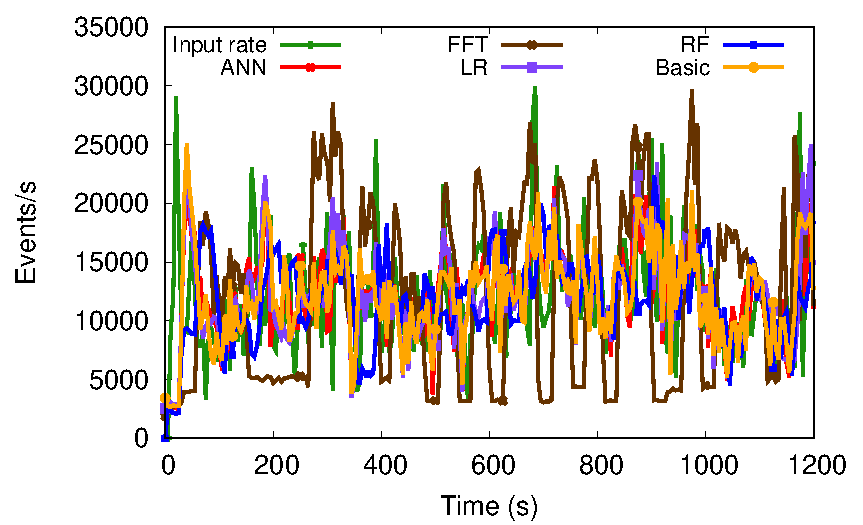
\includegraphics[width=0.75\linewidth]{figures/exp/predictive/TwitterRaw-Throughput.pdf}
     \caption{Throughput of \pSPS{} using \textit{Twitter raw} dataset.}
     \label{fig:exp-pa-twitter-raw-throughput}
\end{figure}

\subsubsection{DNS}
The aim of this experiment is to verify the adaptation ability of \pSPS{} with an input with a different fluctuation than the previous inputs and then analyse the behaviour of it with each predictive model. We used the \textit{DNS} dataset, the \textit{DNS} application, and \textit{Load-Aware grouping} for stream grouping strategy. For calculating the \textit{Saved resources} metric, we have fixed $r_{over} = 12$ (i.e., $r_i = 3$).

\begin{table}[!ht]
\hspace*{-0.5cm}
\centering
\begin{tabular}{|l|llllll|}
\hline \begin{tabular}[c]{@{}l@{}}Pred.\\ Model\end{tabular} & \begin{tabular}[c]{@{}l@{}}Saved\\ Resources\end{tabular} & \begin{tabular}[c]{@{}l@{}}Throughput\\ Degradation\end{tabular} & \begin{tabular}[c]{@{}l@{}}Diff. Proc.\\ Events\end{tabular} & \begin{tabular}[c]{@{}l@{}}Latency\\ (ms)\end{tabular} & \begin{tabular}[c]{@{}l@{}}Error Est.\\ Input\end{tabular} & \begin{tabular}[c]{@{}l@{}}Error Est.\\ Replica\end{tabular}\\ \hline \hline
ANN         & 0.515   & 0.381 & 0.998 & 446.840 & 0.294 & 0.872\\ \hline
FFT         & 0.498   & 0.337 & 0.995 & 397.140 & 0.367 & 1.674\\ \hline
LR          & 0.561   & 0.350   & 1.000    & 464.010 & 0.216 & 0.714\\ \hline
RF          & 0.608   & 0.436  & 0.975 & 545.910 & 0.112 & 0.583\\ \hline
Basic       & 0.604   & 0.511 & 0.984 & 487.600  & 0.090 & 0.738\\ \hline
\end{tabular}
\caption{System metric values of \pSPS{} using different predictive models using \textit{DNS} dataset.}
\label{tab:exp-pa-dns}
\end{table}

Table \ref{tab:exp-pa-dns} summarizes the obtained results. The processing capability of \pSPS{} is confirmed since each proposed model has none or a negligible difference in the number of processed events. The highest difference percentage is around of $2.5\%$ (RF) when compared to \textit{LR}.

Figure \ref{fig:exp-pa-dns-throughput} shows both the input rate and the throughput. Despite the high dynamics of the input rate, \pSPS{} is able to adapt its number of resources in order to process the largest number of events in each time interval.
In this experiment, the model with the best performance is \textit{FFT}, having the lowest value of latency and throughput degradation. On the contrary, the input prediction error is the highest. Considering the values of saved resources, we can conclude that there was an overestimation of the input which led to an overestimation of resources as shown in Figure \ref{fig:exp-pa-dns-replicas}.
If a model with lower resource utilisation is required, \textit{RF} is a good choice, given that it has a difference of $22.08\%$ of the saved resources value with respect to \textit{FFT}. It is worth remarking that due to the above difference, \textit{FFT} throughput degradation and latency decrease by $29.37\%$ and $27.25\%$ respectively.

\begin{figure}[!ht]
    \centering
    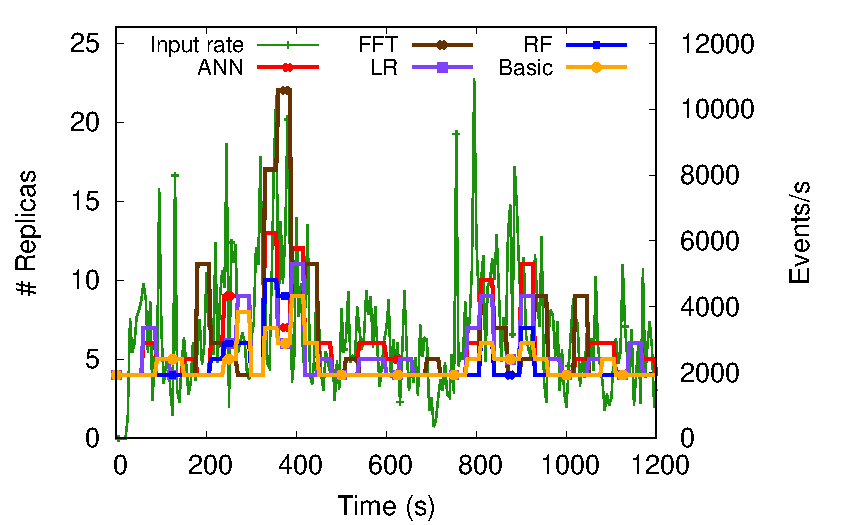
\includegraphics[width=0.75\linewidth]{figures/exp/predictive/DNS-Replicas.pdf}
    \caption{Total number of replicas of \pSPS{} using \textit{DNS} dataset.}
    \label{fig:exp-pa-dns-replicas}
\end{figure}

\begin{figure}[!ht]
    \centering
    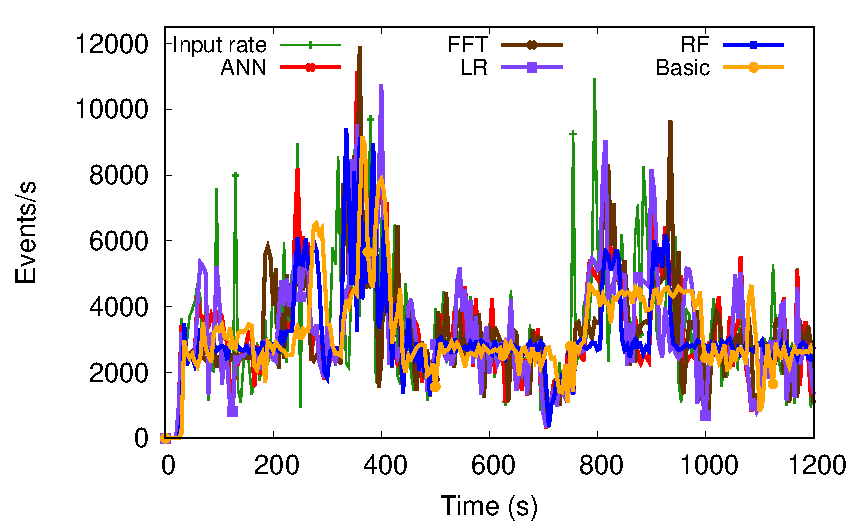
\includegraphics[width=0.75\linewidth]{figures/exp/predictive/DNS-Throughput.pdf}
    \caption{Throughput of \pSPS{} using \textit{DNS} dataset.}
    \label{fig:exp-pa-dns-throughput}
\end{figure}

\subsubsection{Log}
We used the \textit{Log} dataset, the \textit{Log} application, and \textit{Load-Aware grouping} for stream grouping strategy. For calculating the \textit{Saved resources} metric, we have fixed $r_{over} = 32$ (i.e., $r_i = 8$).

\begin{table}[!ht]
\centering
\begin{tabular}{|l|llllll|}
\hline \begin{tabular}[c]{@{}l@{}}Pred.\\ Model\end{tabular} & \begin{tabular}[c]{@{}l@{}}Saved\\ Resources\end{tabular} & \begin{tabular}[c]{@{}l@{}}Throughput\\ Degradation\end{tabular} & \begin{tabular}[c]{@{}l@{}}Diff. Proc.\\ Events\end{tabular} & \begin{tabular}[c]{@{}l@{}}Latency\\ (ms)\end{tabular} & \begin{tabular}[c]{@{}l@{}}Error Est.\\ Input\end{tabular} & \begin{tabular}[c]{@{}l@{}}Error Est.\\ Replica\end{tabular}\\ \hline \hline
ANN   & 0.603  & 0.236 & 0.987 & 905.290  & 0.355 & 0.537 \\ \hline
FFT   & 0.503  & 0.572  & 1.000 & 9184.060 & 0.746 & 1.191 \\ \hline
LR    & 0.565 & 0.252 & 0.994 & 1021.800  & 0.412  & 0.413 \\ \hline
RF    & 0.661 & 0.335 & 0.998 & 1673.560 & 0.243 & 0.394 \\ \hline
Basic & 0.655 & 0.306 & 0.989 & 855.970  & 0.250 & 0.449 \\ \hline
\end{tabular}
\caption{System metric values of \pSPS{} using different predictive models using \textit{Log} dataset.}
\label{tab:exp-pa-log}
\end{table}

Table \ref{tab:exp-pa-log} summarizes the obtained results. The processing capacity of \pSPS{}  is once again confirmed, where each proposed model has a none or a negligible difference of processed events and the highest difference percentage of events processed is around of $1.52\%$ (\textit{ANN}).
\textit{Basic} presents the best performance, both in terms of resource usage and latency. Figure \ref{fig:exp-pa-log-replicas} shows the amount of used replicas, where we can observe that the amount used by \textit{Basic} does not vary much. Although there are high peaks of the input rate (see Figure \ref{fig:exp-pa-log-throughput}), as in $t=700s$, they are short for periods. Thus, it is more appropriate to use a constant amount of replicas rather than to adapt the SPS many times according to the input rate behaviour.

\begin{figure}[!ht]
    \centering
    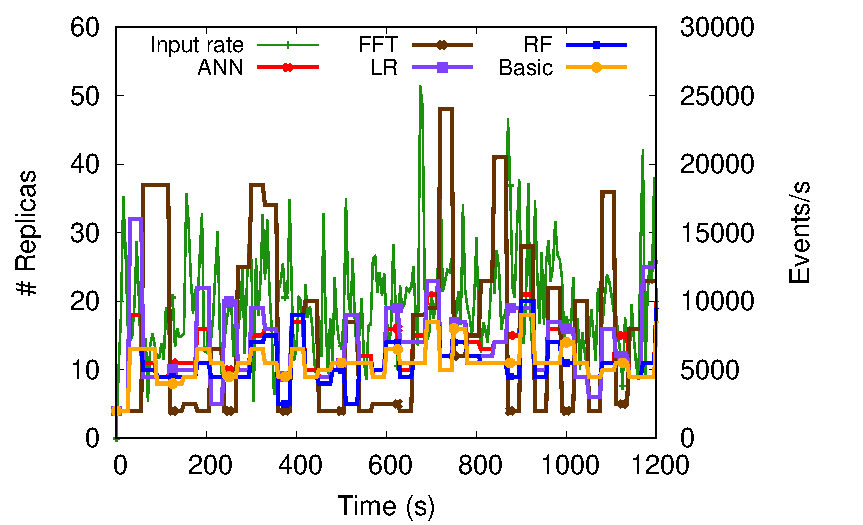
\includegraphics[width=0.75\linewidth]{figures/exp/predictive/Log-Replicas.pdf}
    \caption{Total number of replicas of \pSPS{} using \textit{Log} dataset.}
    \label{fig:exp-pa-log-replicas}
\end{figure}

\begin{figure}[!ht]
    \centering
    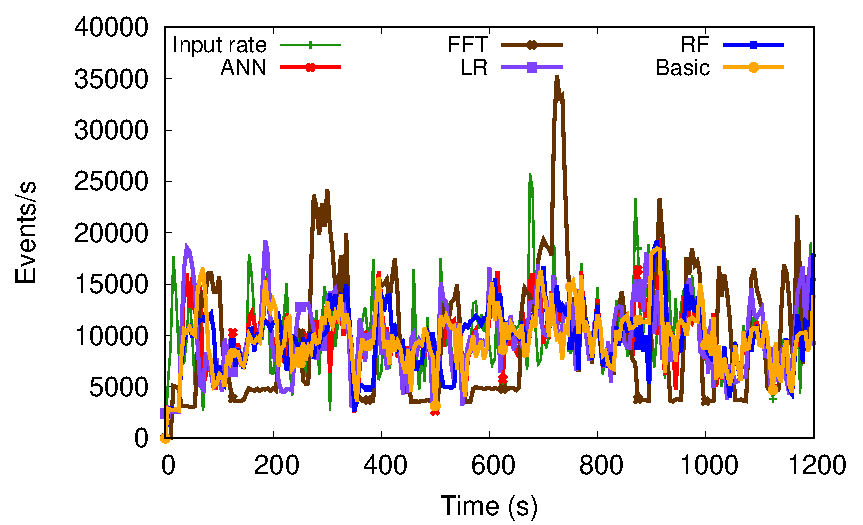
\includegraphics[width=0.75\linewidth]{figures/exp/predictive/Log-Throughput.pdf}
    \caption{Throughput of \pSPS{} using \textit{Log} dataset.}
    \label{fig:exp-pa-log-throughput}
\end{figure}

\subsection{Discussion}
In this section, we have seen the importance of the parameters, because depending on the size of the time interval, it increases or decreases the latency of the SPS.

Compared to \textit{DABS}, evaluation results confirm the effectiveness of the dynamic replica adaptation of \pSPS{}. In the experiments, latency decreases by $74.44\%$ and saved resources increase $19.94\%$, when compared to \textit{DABS}. 

On the other hand, we observed that the most appropriate predictor model depends on the type of input rate behavior. In this way, we also corroborated that our solution is able to adapt to different types of applications and datasets.